\subsection{Método}

Segundo \citeonline{php5ConceitosProgramacaoEIntegracaoComBancoDeDados}, um
método pode ser definido como sendo as operações que manipulam os dados de uma
classe, ou seja, definem o que as classes podem e sabem fazer, como por exemplo
acelerar um carro modificando o valor de sua propriedade chamada
\textit{velocidade} para um valor crescente em um determinado espaço de tempo.

Conforme descrito por \citeonline{c++ComoProgramar}, os métodos também podem ser
chamados de funções membro de uma classe. Perante este esclarecimento, se
comparado a programação estruturada, um método pode ser considerado como
sendo uma função que pertence a uma classe \cite{programmingPhp}.

\begin{figure}[h!tb]
	\caption{Criação de um método utilizando a linguagem PHP}
	\label{fig:metodo}

	\centering
	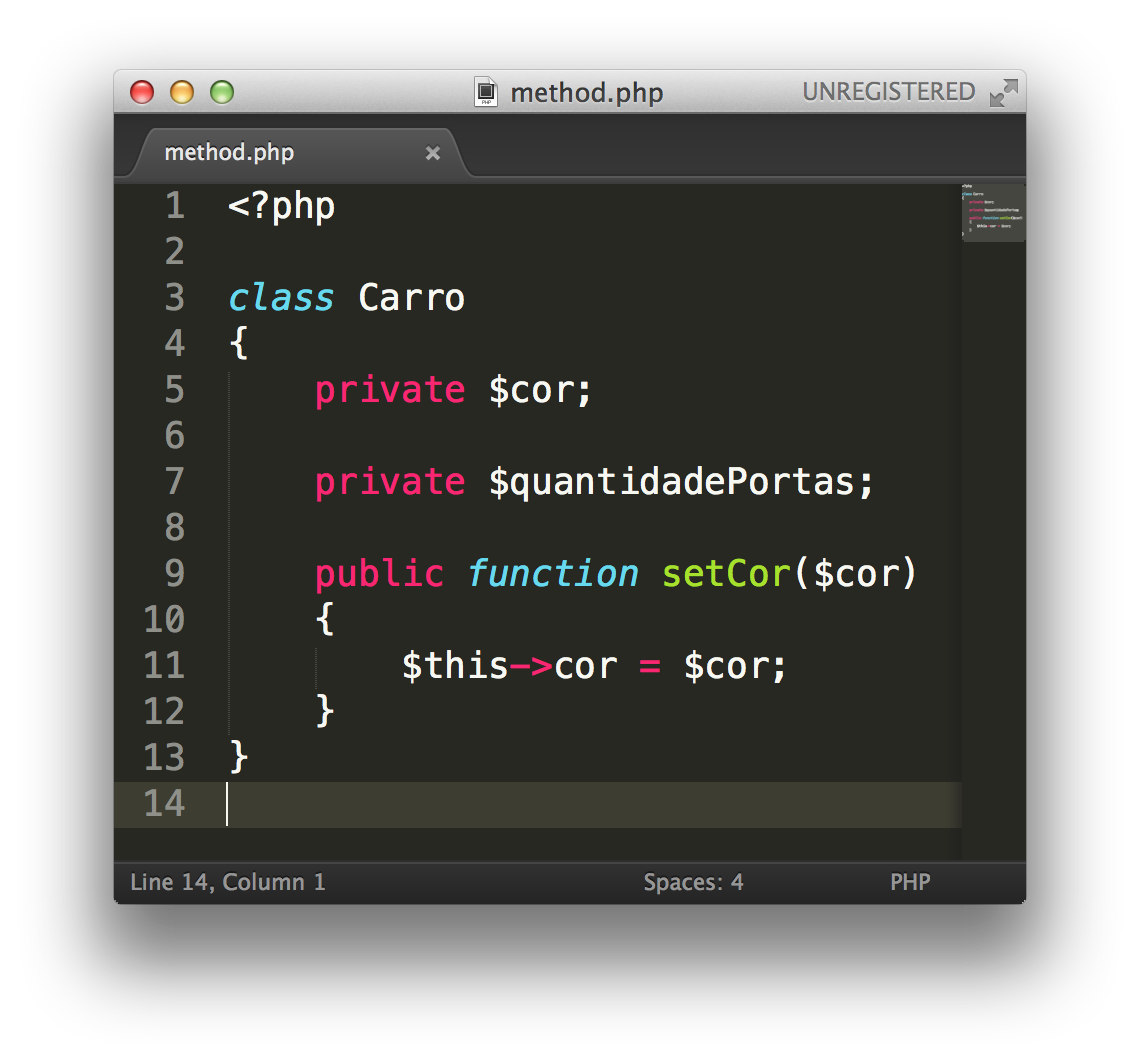
\includegraphics[width=0.68\textwidth]{images/method.png}

	\centering
	\footnotesize Fonte: \fonteOAutor
\end{figure}

\FloatBarrier 	% Este comando impede que as imagens
				% flutuem a partir deste ponto no seu documento

Na sequência, você irá conferir uma explicação referente ao código que foi
apresentado na Figura \ref{fig:metodo}:

\begin{alineas}
    \item linha 1: vê-se o início da execução de um bloco de código PHP;
    \item linha 3: define-se uma classe chamada \textit{Carro};
    \item linha 4: informa-se onde inicia o bloco de uma classe;
    \item linha 5 e 7: cria-se duas propriedades para a classe
    \textit{Carro};
    \item linha 9: é solicitado para que o interpretador crie um método
    cuja visibilidade seja pública e define-se que este método será identificado
    pelo nome \textbf{setCor}.
    Além disso, informa-se que este método deve receber um parâmetro (um valor
    que  irá configurar a propriedade de uma classe);
    \item linha 10: define-se onde inicia o bloco cujo escopo
    corresponda ao método \textbf{setCor};
    \item linha 11: utilizou-se uma variável especial chamada
    \textbf{\$this}, esta variável permite acessar qualquer propriedade ou
    método dentro da própria classe ou \textit{superclasse}; depois, usou-se
    o operador de acesso a um objeto (representado pelo símbolo \textbf{->}); em
    seguida, informa-se ao interpretador do \acs{PHP}, a necessidade de
    manipular o valor da propriedade \textit{cor}, sendo que, ela deverá receber o valor
    informado como parâmetro para o método \textbf{setCor};
    \item linha 12: define-se onde termina o bloco que corresponde ao
    método \textbf{setCor};
    \item linha 13: informa-se o encerramento do bloco de uma classe.
\end{alineas}

Como foi visto o conceito de métodos a seguir será apresentado o conceito de
propriedades.
